\label{vascularModel}

\begin{figure*}[t]
 \begin{center}
  \begin{tabular}{m{6cm}m{6cm}}
   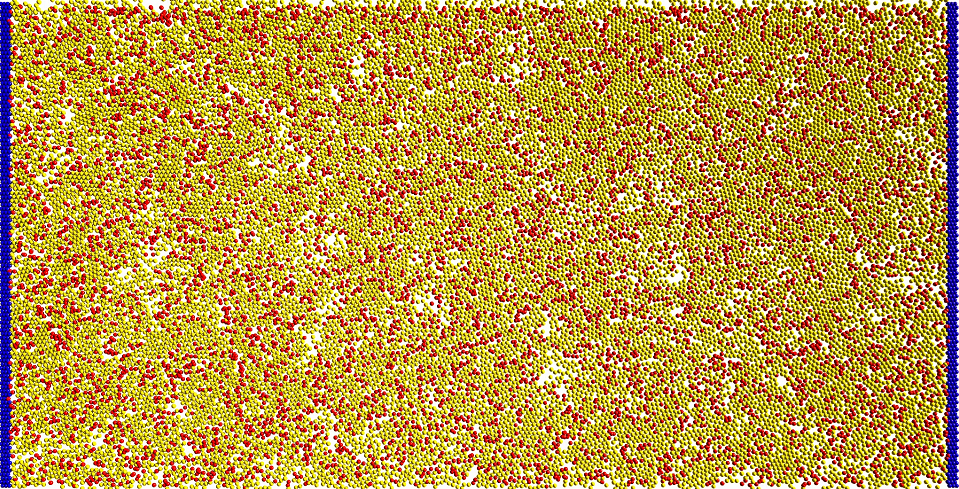
\includegraphics[width=5.9cm]{./figures/init_state.png} &
   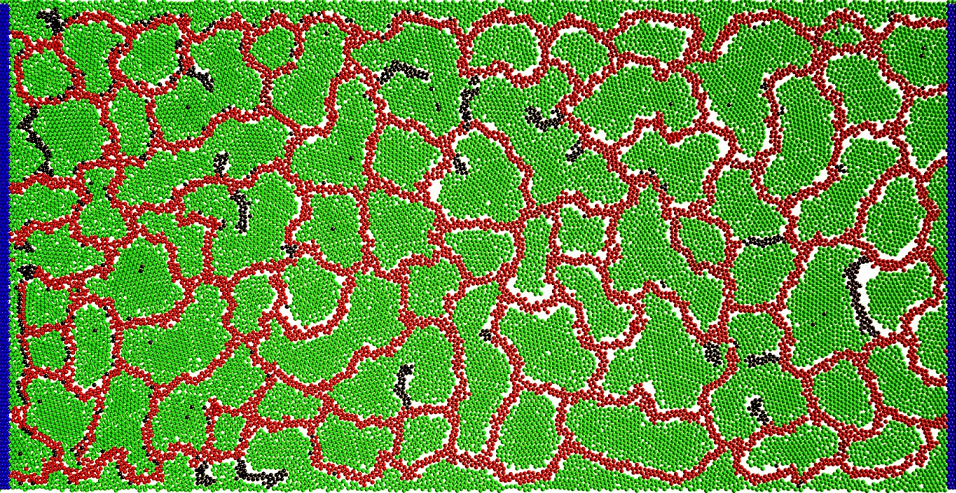
\includegraphics[width=5.9cm]{./figures/vessel30.png}\\
   (a) Initial random distribution & (b) Stable vascular network \\
   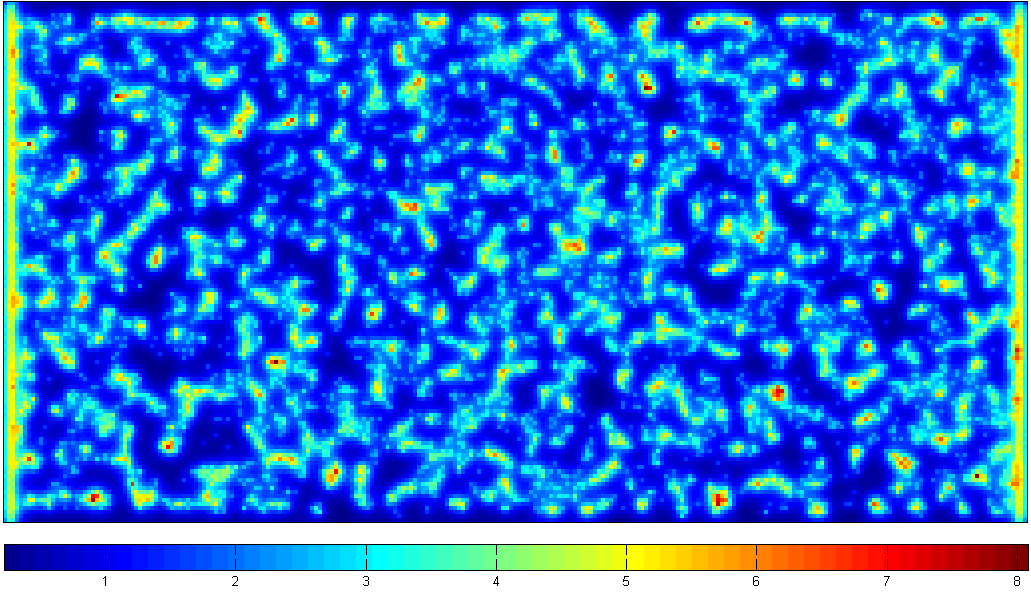
\includegraphics[width=5.9cm]{./figures/Chemo_init_state.png} \hspace{50mm} &
   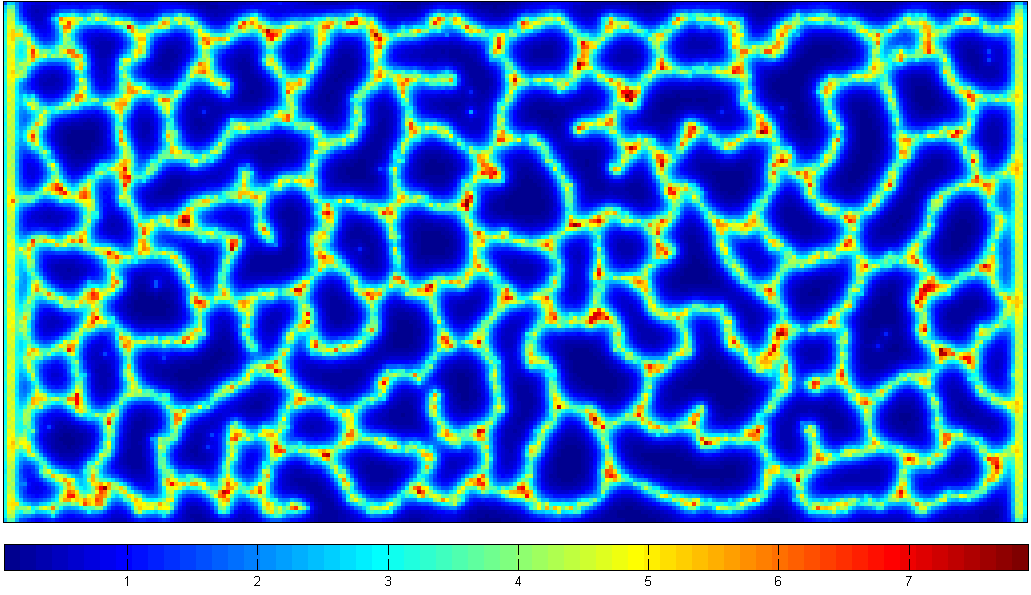
\includegraphics[width=5.9cm]{./figures/Chemo_steady_state.png} \hspace{50mm}\\
   (c) Chemoattractant during formation & (d) Chemoattractant state distribution \\
   \end{tabular}
   \end{center}
 \caption{\textbf{Self-organizing Network}: (a) is the initial conditions with fixed circulatory cells (blue) on each side and vascular (red) and supported cells (yellow) randomly mixed; (b) is the steady state network following self organization; (c) is the distribution of chemoattractant during vessel formation and (d) is at a steady state. In all images of biochemical distribution, blue signifies a low concentration, while red signifies a high concentration.}
 \vspace{+1mm}
\label{phaseOne}
\end{figure*} 

At this proof-of-concept stage, a two-dimensional model was constructed and evaluated. Figure~\ref{phaseOne}(a) illustrates the initial state of the simulated cell culture. Vessel cells (blue) that simulate the external circulatory system are arranged in two columns on both sides of the cell culture area. The left column represents the source, and the right column represents the sink, in parallel to the arterial-venous network architecture in vertebrates \cite{delindavis:arterialvenoussystems}.

The tissue to be supported by the vascular network is simplified to be a field of identical cells, referred to as supported cells (yellow), randomly distributed across the area in between the two circulatory cell columns. Mixed within this field of supported cells are vascular cells (red), similar  to the endothelial cells in vertebrates \cite{delindavis:Merks2008ContactInhibited}. It is the mechanisms of the vascular cells that are to be optimized by the genetic algorithm.

During simulation, the randomly distributed vascular cells self-organize and can form a vascular network connected to both columns of circulatory cells. If this process succeeds, the supported cells will form clusters contained within each network lacuna. An example of a self-organized network is illustrated in Figure~\ref{phaseOne}(b). This developmental process is described in more detail in Section~\ref{vesselDevelopment}.

To evaluate the performance of the network, first an estimate of the flow through the vascular system is calculated and then the vascular network operation is simulated. As the network provides nutrients, the supported cells become active (turn green in the figures) and consume nutrients and secrete wastes. Note that in this case the network fitness would be high because almost all of the supported cells are active and close to a vessel. This network operational process is described in more detail in Section~\ref{fitnessFunction}.

\subsection{De Novo Vascularization Model}
\label{vesselDevelopment}

The two key cellular mechanisms in vascularization are chemotaxis, where cells move in respond to chemical gradients, and tight junctions, where adjacent cells form strong bonds.  Cells are modeled as particles that can secrete and respond to chemicals and move in response to forces. The modeling framework is based on iDynamics \cite{Lardon2011IDynoMiCS} originally created for biofilm models.

Initially, the particles representing epithelial cells are placed randomly in the simulation domain mixed with the support cells.  A chemotactic nutrient is initially supplied at concentration $N_{c}$, set at $8.9 \times 10^{-8} m^{-2}$.  The fixed cells on the sides of the cell culture secrete $C_{long}$, a chemoattractant with small decay rate, and $C_{short}$, a chemoattractant with a large decay rate. The moving cells within the culture only secrete $C_{short}$. The decay rates affect the shape of the chemoattractant gradient. $C_{short}$ is a localized concentration with a sharp gradient, and $C_{long}$ has a long-distance shallow gradient.  The concentrations of each are described by the Monod-kinetic reaction in Equation \ref{chemoattractantsecretion}.  $D_{c}$ of both chemoattractants are set to $1 \times 10^{-13} m^{2} s^{-1}$ as given in the \text{in-vitro} angiogenesis study of Merks et al \cite{delindavis:Merks2008ContactInhibited}; $\beta$ is the decay rate; $M$ is the mass of the secreting cell; $k$ is the Monod-kinetic coefficient; $\mu$ is the maximum secretion rate.

\begin{equation}
\frac{\partial C}{\partial t}=D_{c}\bigtriangledown^{2} C + \mu \frac{N_c}{(N_c +k)} M - \beta C
\label{chemoattractantsecretion}
\end{equation}

The moving cells respond to the gradient of the chemoattractants by tending to towards higher concentrations in a process described in Equation 2 and by Adler \cite{delindavis:chemotaxisbasepaper}. Let $p$ be a particle that responds to chemoattractant $C$. A random unit vector $\vec{c}$ is generated and considered as a potential chemotactic force on $p$. The local gradient of chemoattractant across $p$ in direction $\vec{c}$ is determined by sampling $C$ ahead of $p$, referred to as $C^{+}$, and behind $p$, referred to as $C^{-}$. The magnitude of force $F$ in direction $\vec{c}$ is given by the equation \ref{chemotaxis} \cite{delindavis:Merks2008ContactInhibited}, where $\lambda$ is the parameter that controls the magnitude of the response to the gradient and $\alpha$ controls saturation of the chemotactic force. The force $F$ is only applied to the particle if greater than zero.

\begin{equation}
F = \lambda \Big(\frac{C^{+}}{1 + \alpha C^{+}} - \frac{C^{-}}{1 + \alpha C^{-}}\Big)
\label{chemotaxis}
\end{equation}



Adhesive forces act among the particles and are attractive at close distances and neutral otherwise. In this work, endothelial cell-cell adhesion is strong and endothelial-supported cell is weak. When endothelial cells become close, tight junctions begin to form, binding the cells together as a precursor to vessel construction. In the model, if two adjacent cells form a tight junction, then a stiff spring connects the corresponding particles.

In addition to chemotactic force $F \cdot \vec{c}$, each particle experiences forces due to non-overlapping constraints caused by competition for space. Once the net forces have been assigned to each particle, the system is relaxed by a shoving algorithm which moves the particles along their force vectors to minimize stress. In this way, the vessel particles push through the supported particles, form clumps due to attractive chemotactic forces, and then buckle and extend immature vessels. The system can eventually reach the morphology illustrated in Figure~\ref{phaseOne}(b), in which all biomechanical forces are relaxed, and concentrations of molecules are stable, see Figure~\ref{phaseOne}(d).

\begin{table}[ht]
\caption{Known parameter descriptions} % title of Table
\centering
\begin{footnotesize}
\begin{tabular}{l l l}
\hline
Parameter   &  Value & Description\\ \hline \hline
%\\ [1ex]      % [1ex] adds vertical space
$D_{c}$     & $1 \times 10^{-13} m^{2} s^{-1}$ & Chemoattractant Diffusion coefficient \\%% value verified - cgl
$N_{c}$     & $3 \times 10 g L^{-1}$ & Chemoattractant nutrient concentration \\%% value verified - cgl
$M_{fixed}$  & $1 \times 10^{-11} g$ & Mass of fixed epithelial cells \\%% value verified - cgl
$M_{moving}$  & $1 \times 10^{-11} g$ & Mass of moving epithelial cells \\%% value verified - cgl
$\alpha $     &  $0.1$           & Saturation of chemotactic force\\
[1ex]      % [1ex] adds vertical space

\hline
\end{tabular}
\end{footnotesize}
\label{parameters}
\end{table}
